\chapter{記分板設計}
%\renewcommand{\baselinestretch}{10.0} %設定行距
\section{設計概念}
    依老師要求採用機械轉盤傳動計分系統,由齒輪帶動個位數及十位數的數字轉盤,再搭配程式驅動,使其能夠輕鬆且準確的計算分數,圖為我們自己製作的計分板。(圖.\ref{messageImage_1685927228163})\\
    
\begin{figure}[hbt!]
\center
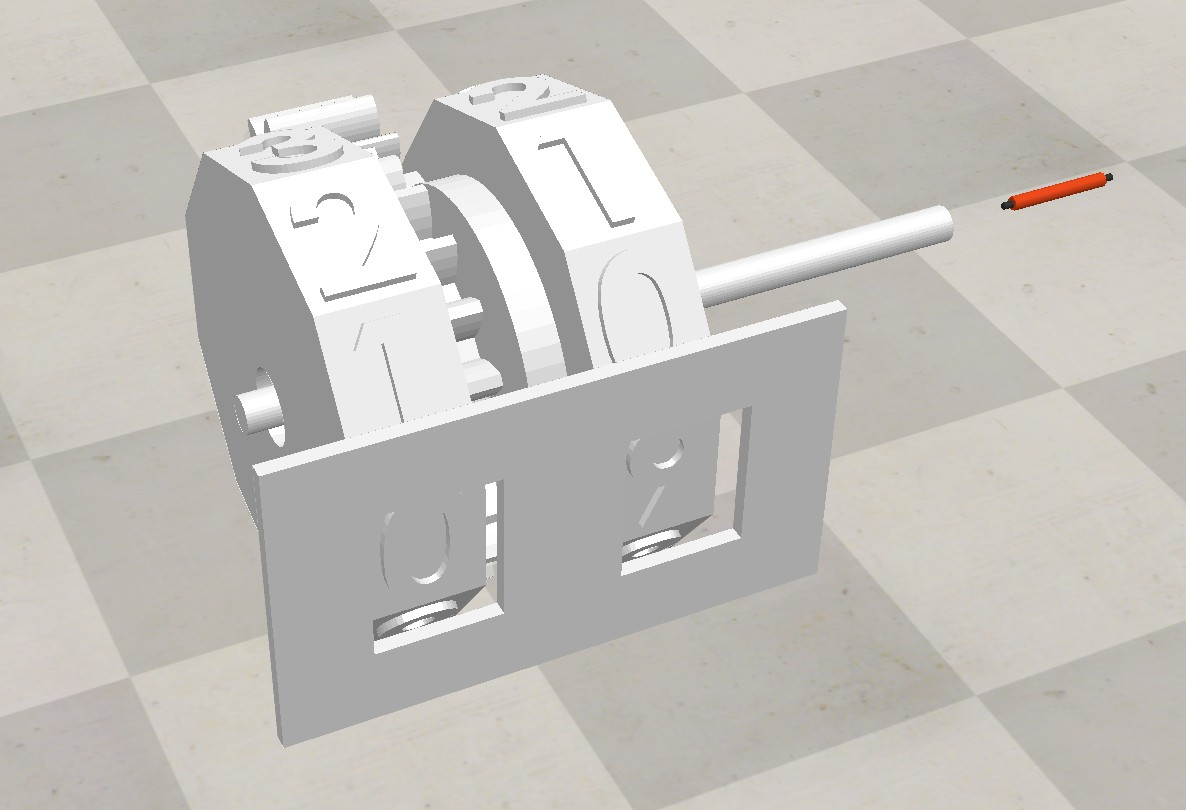
\includegraphics[width=13cm]{messageImage_1685927228163}
\caption{\Large 機械轉盤傳動計分系統}
\label{messageImage_1685927228163}
\end{figure}
    
\section{製作過程}

模型是用SOLIDWORKS繪製,先將各個零件分別繪製,再依序組合完成,最後轉到CoppeliaSim預備模擬。數字輪盤的設計是將圓盤的曲面切割成數個平面並放上數字,齒輪則是經過相關數據的計算完成的,我們有再多製作一個面板使這個計分系統上的得分數更方便閱讀。\\
剛開始搜尋資料時很快就理解了它的運作原理,還認為計分板的繪製不太困難,實際下手畫圖才發現其實有很多細節需要注意,尤其是齒輪的嚙合需要更精細。其中遇到最大的瓶頸,是將SOLIDWORKS裡呼叫的標準零件放進組合圖容易自動跳回標準尺寸,以至於個位數齒輪的齒數繪製不易。且因尚未解決此問題,只能趁SOLIDWORKS檔還是我們所要的形狀時趕緊轉成stl檔到CoppeliaSim做程式設計。\\







